\documentclass{beamer}
\usepackage[french]{babel}
\usepackage{beamerthemesplit} % new 
\usepackage[utf8]{inputenc}
\usepackage{tabularx} % in the preamble
\usepackage{listings}
\usetheme{Warsaw}
\begin{document}
\lstset{
	tabsize=4,
	language=Java,
        basicstyle=\scriptsize,
        columns=fixed,
        extendedchars=true,
        breaklines=true,
		frame=single,
        showtabs=false,
        showspaces=false,
        showstringspaces=false,
        identifierstyle=\ttfamily,
        keywordstyle=\color[rgb]{0,0,1},
        commentstyle=\color[rgb]{0.133,0.545,0.133},
        stringstyle=\color[rgb]{0.627,0.126,0.941},
        numbers=left, 
        numberstyle=\tiny,
        xleftmargin=\parindent
}

\title{Technologies mobiles} 
\author{Olivier Levitt} 
\date{\today} 
\AtBeginSubsection[]
{
  \begin{frame}
  \frametitle{Contents}
  \tiny{\tableofcontents[currentsubsection]}
  \end{frame}
}


\frame{
\titlepage
\begin{center}

\includegraphics[width=60pt]{google-android.jpg}

\includegraphics[width=60pt]{ios.png}

\includegraphics[width=60pt]{wp8.jpg}

\includegraphics[width=60pt]{bb10.jpg}
\end{center}
} 

\frame{\frametitle{Sommaire}\tableofcontents} 
 
\section{Présentation et objectifs du cours}
\subsection{Organisation administrative}
\frame{
\frametitle{Planning}
\begin{itemize}
  \item{30 janvier : 3h de cours, 3h de TP}
  \item{6 février : 3h de cours}
  \item{13 février : 6h de TP}
  \item{Validation des sujets de projet avant le 20 février}
  \item{20 février : 6h de TP dédiées au projet}
  \item {? mars : Soutenance du projet}
\end{itemize}
}
\frame{
\frametitle{Evaluation}
\begin{itemize}
  \item{Projet : création d'une application}
  \item{Groupe de 2}
  \item{Sujet ``libre''}
  \item{6h de TP dédiées au projet + travail personnel}
  \item{Soutenance / Présentation de l'application}
\end{itemize}
}
\subsection{Contexte et objectifs}
\frame{
\frametitle{Contexte et objectifs}
\begin{itemize}
  \item Smartphones, tablettes et assimilés (TV, montre, autoradio, consoles de
  jeu \ldots)
  \item Dev d'application, pas de dev de la plateforme
  \item 1ère partie : le dev mobile en général
  \item 2ème partie : application sous android
\end{itemize}
}

\section{Le développement mobile} 
\subsection{Spécificités du développement mobile}
\frame{
\frametitle{Des appareils suréquipés}
\begin{itemize}
  \item Téléphonie (SMS, MMS, appels)
  \item Internet (GPRS, EDGE, 3G, 4G, WIFI)
  \item Réseaux locaux (Bluetooth, réseaux adhoc, NFC)
  \item Capteurs (Luminosité, proximité)
  \item Localisation (GPS, triangulation, SSID wifi)
  \item Notifications (Vibreur, haut-parleurs, LED)
  \item Photo / vidéo
  \item Stockage de données (Mémoire flash, SD externe, SQLite)
  \item Interactions (Ecran tactile, gestures, boutons physique)
  \item Et encore d'autres \ldots
\end{itemize}
Et des API pour utiliser tout ça !
}
\frame{
\frametitle{Des contraintes techniques importantes}
\begin{itemize}
  \item Processeur
  \item Mémoire RAM
  \item Stockage de données
  \item Gestion de la batterie
  \item Stabilité et débit de la connexion internet
  \item Cycle de vie de l'application
  \item Taille d'écran 
  \item Inputs atypiques (clavier virtuel, gestures, peu de boutons \ldots)
\end{itemize}
Contraintes à garder en tête en permanence.
}
\frame{
\frametitle{La fragmentation}
Une application publiée sur le google playstore cible plus de 2400 appareils
différents !\\
\begin{itemize}
   \item ``Write once, run everywhere'' ?
   \item Comment tester / débugger pour tous ces appareils ?
  \item Eviter de géner l'utilisateur (versions HD, appareils non compatibles)
  \item S'adapter quand une fonctionnalité n'est pas disponible
\end{itemize}
}
\frame{
\frametitle{La fragmentation, taille d'écran}
Comment gérer toutes les tailles d'écran ? 
\begin{itemize}
  \item Montres connectées : de 1 à 2 pouces
  \item Smartphones lowcost : 3 pouces (Galaxy pocket, galaxy Y)
  \item Smartphones high-end : 4 à 5 pouces (IPhone 5, HTC 8X, nexus 4)
  \item Phablets : 5 à 6 pouces (Galaxy note, HTC butterfly)
  \item Tablettes : 7 pouces (Nexus 7, IPad mini), 8 pouces (Archos 80g9), 10 pouces (Nexus 10, IPad)
\end{itemize}
}


\frame{
\frametitle{De nombreuses autres sources de fragmentation}
\begin{itemize}
  \item Versions de l'OS
  \item Résolutions d'écran
  \item Elements hardware présents
  \item Puissance
  \item Modifications constructeur / ``rom custom''
  \item \ldots
\end{itemize}
}
\frame{
\frametitle{Des Ecosystèmes forts}
\begin{itemize}
  \item Obligation d'utiliser le SDK fourni
  \item Suivre les guidelines
  \item Restrictions liées à la plateforme
  \item Utilisation des services de la plateforme
  \item Processus de déploiement des applications
  \item Règles des ``store'' (validation, monétisation \ldots)
\end{itemize}
}
\subsection{Présentation des différents OS mobile}
\frame{
\frametitle{iOS}

\includegraphics[width=60pt]{ios.png}
\begin{itemize}
  \item Soutenu par Apple
  \item Présenté le 9 janvier 2007
  \item Dédié aux produits apple (iPhone, iPad, iPod)
  \item 400 millions d'appareils (Septembre 2012)
  \item Programmation en objective-C, sur mac OS X uniquement
  \item Appstore : validation + 100\$ / an
\end{itemize}
}
\frame{
\frametitle{Android}


\includegraphics[width=60pt]{google-android.jpg}
\begin{itemize}
  \item Soutenu par Google
  \item 1.0 en septembre 2008, 1.5 en avril 2009
  \item Plus de 2400 appareils officiellement supportés, + de 50 constructeurs
  \item 480 millions d'appareils activés (Septembre 2012)
  \item Programmation en JAVA, sur windows / OS X / linux
  \item Open-source
  \item Google playstore : pas de validation + 25\$
\end{itemize}
}
\frame{
\frametitle{Windows phone 8}


\includegraphics[width=60pt]{wp8.jpg}
\begin{itemize}
  \item Soutenu par Microsoft
  \item Présentation au public le 29 octobre 2012
  \item Successeur de windows phone 7 (logique)
  \item Plusieurs constructeurs dont Nokia, HTC et Samsung
  \item Programmation en C\# sur windows 
  \item Windows marketplace : validation + 100\$ / an
\end{itemize}
}
\frame{
\frametitle{Blackberry 10}


\includegraphics[width=60pt]{bb10.jpg}
\begin{itemize}
  \item Soutenu par RIM (Research in motion)
  \item Présentation au public le 30 janvier 2012 (!)
  \item Appareils produits par RIM
  \item C / C++, HTML5, Adobe AIR, Portage android
  \item Blackberry appworld : validation + gratuit
\end{itemize}
}
\frame{
\frametitle{Ubuntu for phones}
\begin{itemize}
  \item Soutenu par Canonical
  \item Teaser le 2 janvier 2012, testable sur galaxy nexus fin février
  \item Premiers ubuntu phones promis pour début 2014
  \item Facilement utilisable sur les téléphones android ?
  \item HTML5, C/C++ + QML
  \item Open-source
  \item Peu d'infos sur le store
\end{itemize}
}
\section{Le développement sur android} 

\subsection{Mise en place}
\frame{
\frametitle{Les marque-page}
\begin{itemize}
  \item www.frandroid.com (actu FR)
  \item www.androidpolice.com (actu EN)
  \item www.androidcentral.com (actu EN)
  \item www.d.android.com (la bible EN)
  \item www.stackoverflow (Q/A EN)
  \item \#android et \#android-dev sur freenode (chat irc EN)
  \item www.breizhjug.org et www.paug.fr (communautés FR)
  \item www.google.fr (réservoir à tutoriels)
\end{itemize}
}
\frame{
\frametitle{Bien commencer}
La programmation android fait partie des plus accessibles :
\begin{itemize}
  \item Des (bonnes) bases de programmation en JAVA
  \item Un ordinateur (Windows, Linux, Mac OS X)
  \item Un appareil android (conseillé, l'émulateur étant \ldots moyen)
\end{itemize}
C'est tout !
}
\frame{
\frametitle{Les niveaux d'API}
\begin{table}
\begin{tabular}{|l|c|c|c|r|}
  \hline
  Version & Nom & API level & Distribution & Cumulé \\
  \hline
  1.5 & Cupcake & 3 & 0\% & 0\% \\
  1.6 & Donut & 4 & 0.2\% & 0.2\% \\
  2.1 & Eclair & 7 & 2.4\% & 2.6\% \\
  2.2 & Froyo & 8 & 9\% & 11.6\% \\
  2.3 & Gingerbread & 9/10 & 47.6\% & 59.2\% \\
  3.X & Honeycomb & 12/13 & 1.5\% & 60.7\% \\
  4.0.X & Ice cream sandwich & 15 & 29.1\% & 89.8\% \\
  4.1 & Jelly bean & 16 & 9\% & 98.8\% \\
  4.2 & Jelly bean & 17 & 1.2\% & 100\% \\
  \hline
\end{tabular}
\caption{\label{s}Répartition des versions pour les accès au google play sur la
dernière quinzaine de 2012}
\end{table}
}
\frame{
\frametitle{Présentation du SDK android}
Téléchargement gratuit : www.d.android.com/sdk
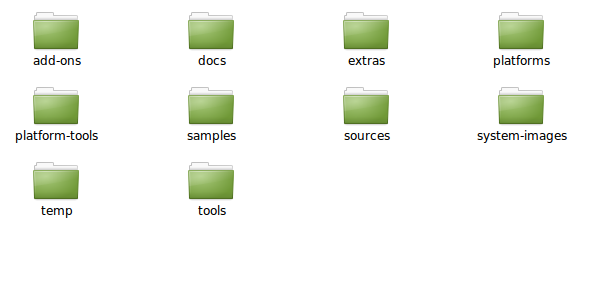
\includegraphics[width=300pt]{sdk.png}
}
\frame{
\frametitle{Présentation du SDK android}
\begin{itemize}
  \item add-ons : Google APIs
  \item docs : Copie de la documentation disponible sur d.android.com
  \item extras : Lib de compatibilité, lib pour les achats in-app \ldots
  \item platform-tools : Binaires de communication avec les appareils android
  (adb, fastboot \ldots)
  \item platforms : 1 dossier par niveau d'API téléchargé
  \item samples : Exemples de projets
  \item sources : Sources de chaque niveau d'API
  \item system-images : Images pour l'émulateur
  \item temp
  \item tools : Outils pour le dev (ddms, apkbuilder, lint \ldots)
\end{itemize}
}
\frame{
\frametitle{Plugin android pour eclipse : ADT}
Installation comme un plugin eclipse classique\\ 
https://dl-ssl.google.com/android/eclipse/\\
ADT fait le lien entre eclipse et le SDK android
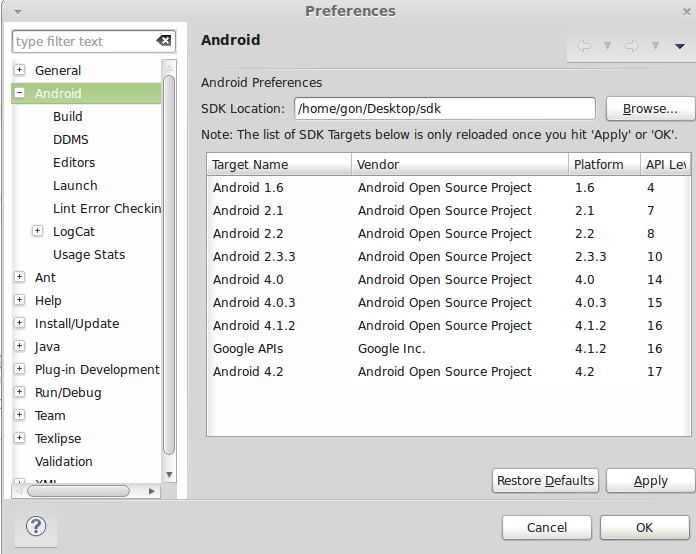
\includegraphics[width=100pt]{adt.png}
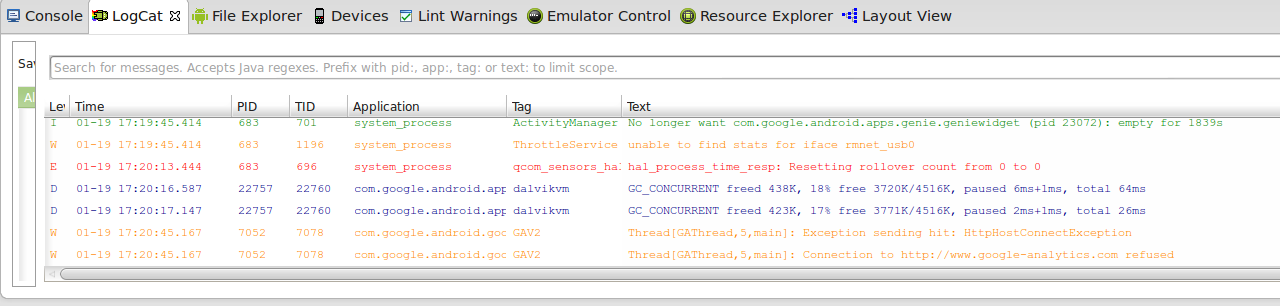
\includegraphics[width=200pt]{views.png}\\\\
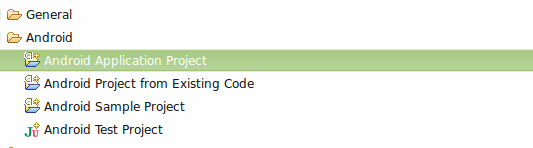
\includegraphics[width=100pt]{project.png}
}
\frame{
\frametitle{L'émulateur}
\begin{itemize}
  \item Utile pour tester certaines configurations
  \item ((très) très) lent
  \item Utiliser un appareil android à la place quand c'est possible
\end{itemize}
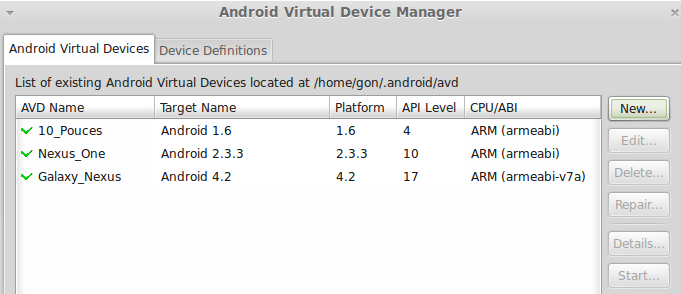
\includegraphics[width=300pt]{avd.png}
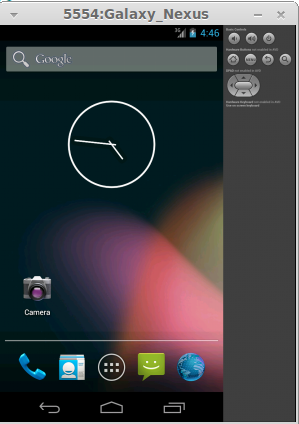
\includegraphics[width=42pt]{emu.png}
}
\frame{
\frametitle{Alternative à l'émulateur}
\begin{itemize}
  \item Problème : émuler de l'ARM sur nos machines x86
  \item Résultat : émulateur ((très) très) lent
  \item Solution proposée : porter android sur x86
  \item http://www.android-x86.org/
\end{itemize}
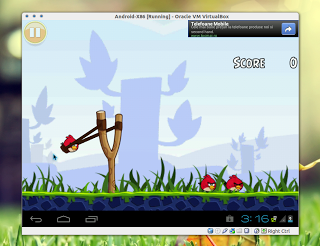
\includegraphics[width=170pt]{x86.png}
}
\frame{
\frametitle{Distribuer l'application}
\begin{itemize}
  \item Une application android = un APK (+/- équivalent d'un jar)
  \item Création et signature de l'APK simple sous eclipse
  \item Distribution directe de l'APK (ex : pour tester, béta fermée)
  \item Publication sur le playstore, 25\$ à l'inscription
  \item Application gratuite ou payante (30\% pour google)
 \end{itemize}
}
\subsection{Architecture}
\frame{
\frametitle{Organisation d'un projet android}
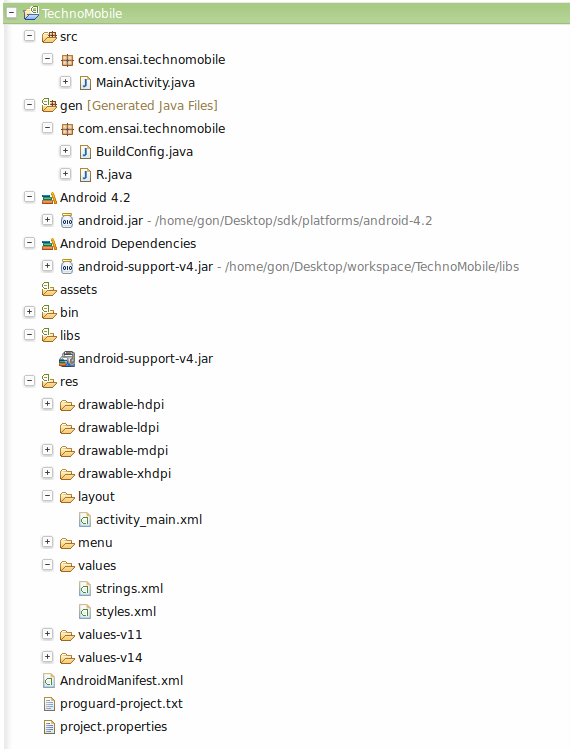
\includegraphics[width=150pt]{structure.png}
}
\frame{
\frametitle{Détail de l'organisation}
\begin{itemize}
  \item src : code source java
  \item gen : identifiants des ressources (généré par le sdk)
  \item Android 4.2 : jar correspondant à l'API cible
  \item Android Dependencies : jar rajoutés, correspond à libs
  \item assets : fichiers fournis avec l'app
  \item bin : résultat de la compilation (dont l'apk)
  \item libs : jar rajoutés
  \item res : ressources (layouts, strings, images \ldots)
  \item AndroidManifest.xml : métadonnées sur l'application, composants,
  permissions \ldots
  \item proguard-project.txt : configuration de proguard
  \item project.properties : généré par le sdk
 \end{itemize}
}
\frame{
\frametitle{AndroidManifest.xml : le coeur de l'application}
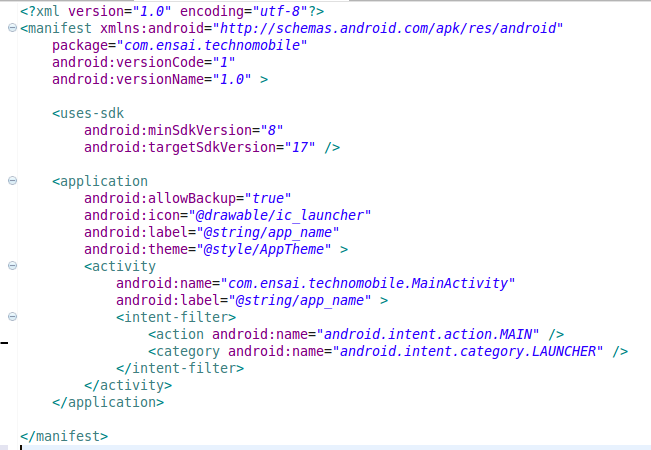
\includegraphics[width=150pt]{manifest.png}
\begin{itemize}
  \item Déclaration des composants
  \item Déclaration des permissions
  \item Analysé par l'OS à l'installation
 \end{itemize}
}
\frame{
\frametitle{Le système de ressources}
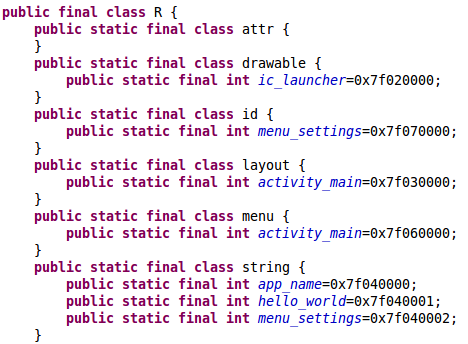
\includegraphics[width=150pt]{ressources.png}
\begin{itemize}
  \item Un identifiant est généré pour chaque ressource (drawable, layout, menu,
  values, style \ldots)
  \item Nom de l'identifiant = nom de la ressource sans l'extension
 \end{itemize}
}
\subsection{IHM}
\frame{
\frametitle{Activity, le composant de base}
  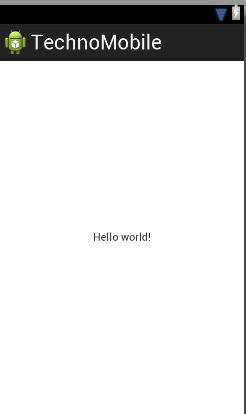
\includegraphics[width=50pt]{activity.png}
\begin{itemize}
  \item 1 activity {\raise.17ex\hbox{$\scriptstyle\sim$}}  un écran
  \item Une application peut avoir 0-n activities
  \item A ajouter dans le manifest
  \item Créer une classe java héritant de Activity 
 \end{itemize}
}
\frame{
\frametitle{Cycle de vie d'une activity} 
  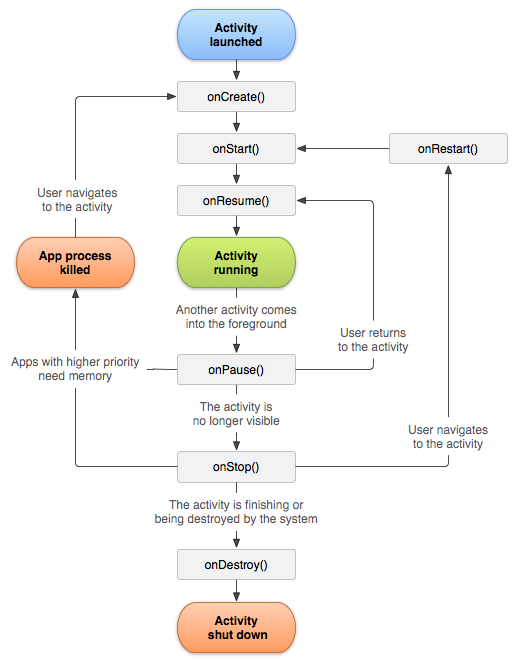
\includegraphics[width=150pt]{activity_lifecycle.png}
}
\begin{frame}[fragile]
\frametitle{Créer une activity : étendre Activity} 
\begin{lstlisting}
public Class MyActivity extends Activity {

	@Override
	protected void onCreate(Bundle savedInstanceState) {
		super.onCreate(savedInstanceState);
		setContentView(R.layout.activity_main);
	}
}
\end{lstlisting}
 \begin{itemize}
 \item onCreate est appellé à la création de l'activity (cf cycle de vie)
 \item appel obligatoire à super.onCreate
 \item le bundle savedInstanceState contient les informations en cas de
 relancement de l'activity
 \item savedInstanceState est null s'il s'agit du premier lancement
 \end{itemize}
\end{frame}
\begin{frame}[fragile]
\frametitle{L'organisation d'une activity : les layouts} 
\begin{lstlisting}
<LinearLayout 
	xmlns:android="http://schemas.android.com/apk/res/android"
    android:layout_width="match_parent"
    android:layout_height="match_parent">

    <TextView
        android:layout_width="wrap_content"
        android:layout_height="wrap_content"
        android:text="@string/hello_world" />

</LinearLayout>
\end{lstlisting}
 \begin{itemize}
 \item Ils sont définis en XML dans le dossier res/layout
 \item Ils définissent l'organisation des vues
 \item Eviter au maximum de modifier / créer les layouts au runtime
 \end{itemize}
\end{frame}
\begin{frame}[fragile]
\frametitle{Les Views}
   Une vue = un élement à l'écran
  \begin{itemize}
    \item TextView = Un texte
    \item EditText = Un champ de texte remplissable
    \item ImageView = Une image
    \item Button
    \item CheckBox
    \item Plein d'autres views de base dans android
    \item Possibilité de créer ses propres views en étendant View ou SurfaceView
 \end{itemize}
\end{frame}
\begin{frame}[fragile]
\frametitle{Les ViewGroups}
  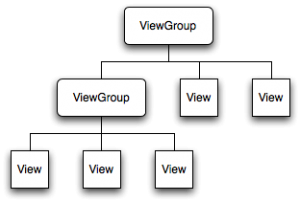
\includegraphics[width=150pt]{viewgroup.png}
  \begin{itemize}
 \item LinearLayout
 \item RelativeLayout
 \item ListView
 \item Plein d'autres
 \item Les vôtres :)
 \end{itemize}
\end{frame}
\begin{frame}[fragile]
\frametitle{Manipuler les éléments de l'UI en java}
Etape 1 : donner un identifiant à la vue
\begin{lstlisting}
<LinearLayout 
	xmlns:android="http://schemas.android.com/apk/res/android"
    android:layout_width="match_parent"
    android:layout_height="match_parent"
    android:id="@+id/monlayout">

    <Button
        android:layout_width="wrap_content"
        android:layout_height="wrap_content"
        android:id="@+id/monbouton"
        android:text="@string/hello_world" />

</LinearLayout>
\end{lstlisting}
\end{frame}
\begin{frame}[fragile]
\frametitle{Manipuler les éléments de l'UI en java}
Etape 2 : récupérer les réferences vers les views
\begin{lstlisting}
public Class MyActivity extends Activity {

	ViewGroup layout = null;
	Button bouton = null;

	@Override
	protected void onCreate(Bundle savedInstanceState) {
		super.onCreate(savedInstanceState);
		setContentView(R.layout.activity_main);
		layout = (ViewGroup) findViewById(R.id.monlayout);
		bouton = (Button) findViewById(R.id.monbouton);
	}
}
\end{lstlisting}
\end{frame}
\begin{frame}[fragile]
\frametitle{Manipuler les éléments de l'UI en java}
\begin{lstlisting}
public Class MyActivity extends Activity {

	ViewGroup layout = null;
	Button bouton = null;

	@Override
	protected void onCreate(Bundle savedInstanceState) {
		super.onCreate(savedInstanceState);
		setContentView(R.layout.activity_main);
		layout = (ViewGroup) findViewById(R.id.monlayout);
		bouton = (Button) findViewById(R.id.monbouton);
	}
	
	public void changerTexte(String texte) {
		bouton.setText(texte);
	}
	
	public void cacherTout() {
		layout.setVisibility(View.INVISIBLE);
	}
}
\end{lstlisting}
\end{frame}
\begin{frame}[fragile]
\frametitle{Ecouter les évenements}
\begin{itemize}
 \item Système de listeners (cf swing)
 \item Il se passe quelque chose sur la vue (touch, focus \ldots) : le listener
 est prévenu
 \item Pour simplifier, sur android on a en général qu'un listener par évenement
 et par view (setXListener au lieu de addXListener sous swing)
 \end{itemize}
\end{frame}
\begin{frame}[fragile]
\frametitle{Ecouter les évenements, guide du bon listener}
Etape 1 : Les interfaces XListener
\begin{lstlisting}
public Interface OnClickListener {
	void onClick(View v);
}
\end{lstlisting}
Etape 2 : Implémenter l'interface
\begin{lstlisting}
public MaClasse implements OnClickListener {
	public void onClick(View v) {
		//Un click a ete fait sur la vue v
	}
}
\end{lstlisting}
\end{frame}
\begin{frame}[fragile]
\frametitle{Ecouter les évenements, guide du bon listener}
Etape 3 : S'enregistrer comme listener
\begin{lstlisting}
public Class MyActivity extends Activity implements OnClickListener {

	Button bouton = null;

    @Override
    protected void onCreate(Bundle savedInstanceState) {
        super.onCreate(savedInstanceState);
        setContentView(R.layout.activity_main);
        bouton = (Button) findViewById(R.id.monbouton);
        bouton.setOnClickListener(this);
    }
	
    public void onClick(View v) {
        //Un Click a ete fait sur la vue v
    }
}
\end{lstlisting}
\end{frame}
\begin{frame}[fragile]
\frametitle{Ecouter les évenements, quelques feintes}
Feinte 1 : Utiliser des listeners anonymes
\begin{lstlisting}
public Class MyActivity extends Activity implements OnClickListener {

    Button bouton = null;

    @Override
    protected void onCreate(Bundle savedInstanceState) {
        super.onCreate(savedInstanceState);
        setContentView(R.layout.activity_main);
        bouton = (Button) findViewById(R.id.monbouton);
        bouton.setOnClickListener(new OnClickListener() {
                public void onClick(View v) {
                //Un Click a ete fait sur la vue v
                }
            });
	    }
}
\end{lstlisting}
\end{frame}
\begin{frame}[fragile]
\frametitle{Ecouter les évenements, quelques feintes}
Feinte 2 : Définir le listener directement dans le layout
\begin{lstlisting}
<LinearLayout 
	xmlns:android="http://schemas.android.com/apk/res/android"
    android:layout_width="match_parent"
    android:layout_height="match_parent"
    android:id="@+id/monlayout">

    <Button
        android:layout_width="wrap_content"
        android:layout_height="wrap_content"
        android:id="@+id/monbouton"
        android:text="@string/hello_world"
        android:onClick="clickSurLeBouton" />

</LinearLayout>
\end{lstlisting}
\begin{lstlisting}
public void clickSurLeBouton(View v) //dans MyActivity
\end{lstlisting}
\end{frame}

\begin{frame}[fragile]
\frametitle{Les intents}
\begin{itemize}
 \item On déclare son intention, android réagit en conséquence
 \item Intents implicites ``Je veux ouvrir la page web https://twitter.com/Ensai35''
 \item ``Je veux envoyer un mail à jlegouic@ensai.fr avec le titre URGENT : FOOT''
 \item Intents explicites ``Je veux lancer l'activity MyActivity''
 \end{itemize}
\end{frame}
\begin{frame}[fragile]
\frametitle{Lancer un intent implicite}
\begin{lstlisting}
public MyActivity extends Activity {
    
    public void envoyerMail() {
        Intent i = new Intent(Intent.ACTION_SEND);
        i.setType("message/rfc822");
        i.putExtra(Intent.EXTRA_EMAIL  , "annee2@ensai.fr");
        i.putExtra(Intent.EXTRA_SUBJECT,"URGENT : FOOT"); 
        i.putExtra(Intent.EXTRA_TEXT   , "...");
        try {
            startActivity(i);
        } 
        catch (ActivityNotFoundException ex) {
            //Pas de client mail installe
        }
    }	
}
\end{lstlisting}
\end{frame}
\subsection{Données}

\end{document}
